\documentclass{article}

\begin{document}
	\section{Dinero Simulator}
		The Dinero simulator is a cache simulator that lets the use experiment with different cache options such as associativity and block size. We modified various options to determine how it affects the cache miss ratio. The 12 main options given to us to test out are listed below. 
		\begin{itemize}
			\item Split cache with 8Byte blocks directally mapped
			\item Split cache with 8Byte blocks 4 way associative
			\item Split cache with 32Byte blocks directally mapped
			\item Split cache with 32Byte blocks 4 way associative
			\item Split cache with 128Byte blocks directally mapped
			\item Split cache with 128Byte blocks 4 way associative
			\item Unified cache with 8Byte blocks directally mapped
			\item Unified cache with 8Byte blocks 4 way associative
			\item Unified cache with 32Byte blocks directally mapped
			\item Unified cache with 32Byte blocks 4 way associative
			\item Unified cache with 128Byte blocks directally mapped
			\item Unified cache with 128Byte blocks 4 way associative
		\end{itemize}
		The split caches were comprised of 16KB instruction cache and 16KB data cache. The unified caches were 32KB large. These experiments were ran using this command for split cache.
		\begin{lstlisting}[language=bash]
			cat ../../project/trace.din | ./dineroIV -l1-dsize \textbf{<DATA_CACHE_SIZE>} -l1-dbsize \textbf{<DATA_BLOCK_SIZE>} -l1-dassoc \textbf{<DATA_ASSOC>} -l1-isize \textbf{<INS_CACHE_SIZE>} -l1-ibsize \textbf{<INS_BLOCK_SIZE>} -l1-iassoc \textbf{<INS_ASSOC>} -informatd
		\end{lstlisting}
		And this command for unified cache.
		\begin{lstlisting}[language=bash]
			cat ../../project/trace.din |  ./dineroIV -l1-usize 32K -l1-ubsize 128 -l1-uassoc 1 -informatd
		\end{lstlisting}
		\par
		The result of the experiment with the dineroIV simulator was consistant with the theroy tought in class. The results are laied neatly in this graoh below. 
		\being{figure}[H]
			\label{uni-cache-metrics}
			\begin{center}
				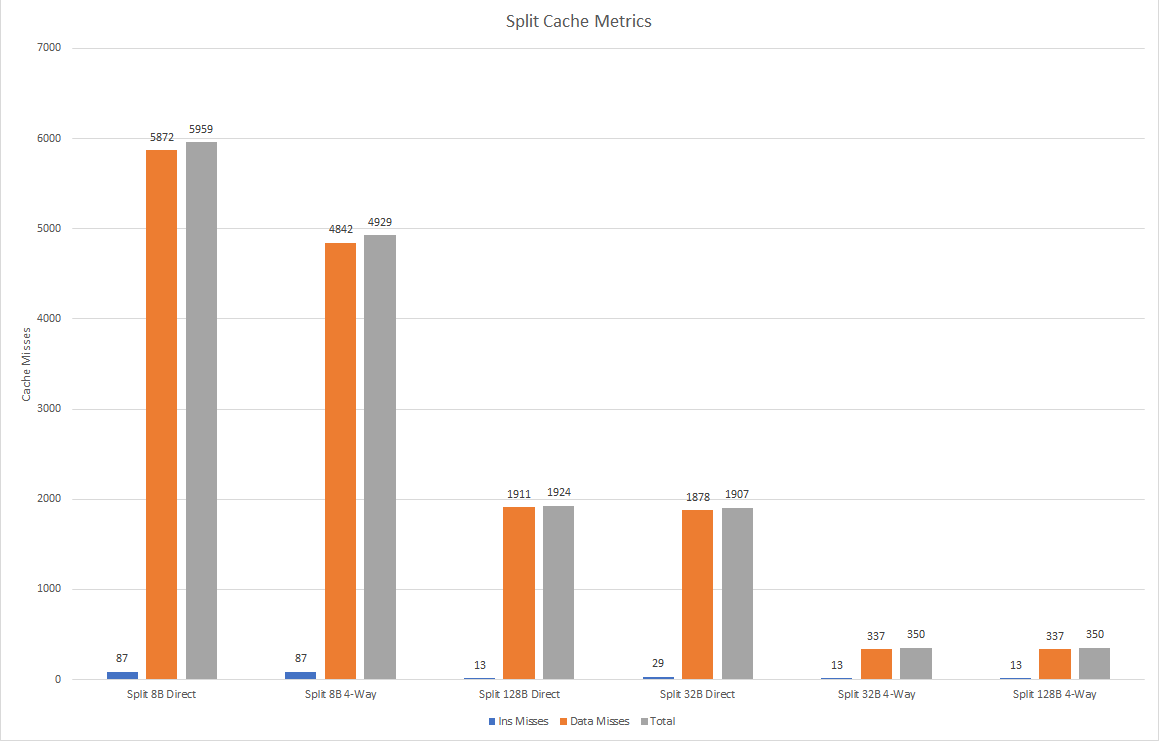
\includegraphics[width=6cm]{uni-cache-metrics.png}
				\caption{Metrics of a unified cache}
			\end{center}
		\end{figure}
\end{document}